Come prima operazione defiano la seguente funzione $f$

\begin{equation}
	f \,:=\, A + B m 
\end{equation}
%
dove B rappresenta il coefficiente angolare della retta, che assumiamo nullo, $m$ la massa applicata al pendolo e A una costante che nel nostro caso è il valore della media pesata dei periodi $\mathcal{T}$.\\

\begin{SCfigure}
    \centering
    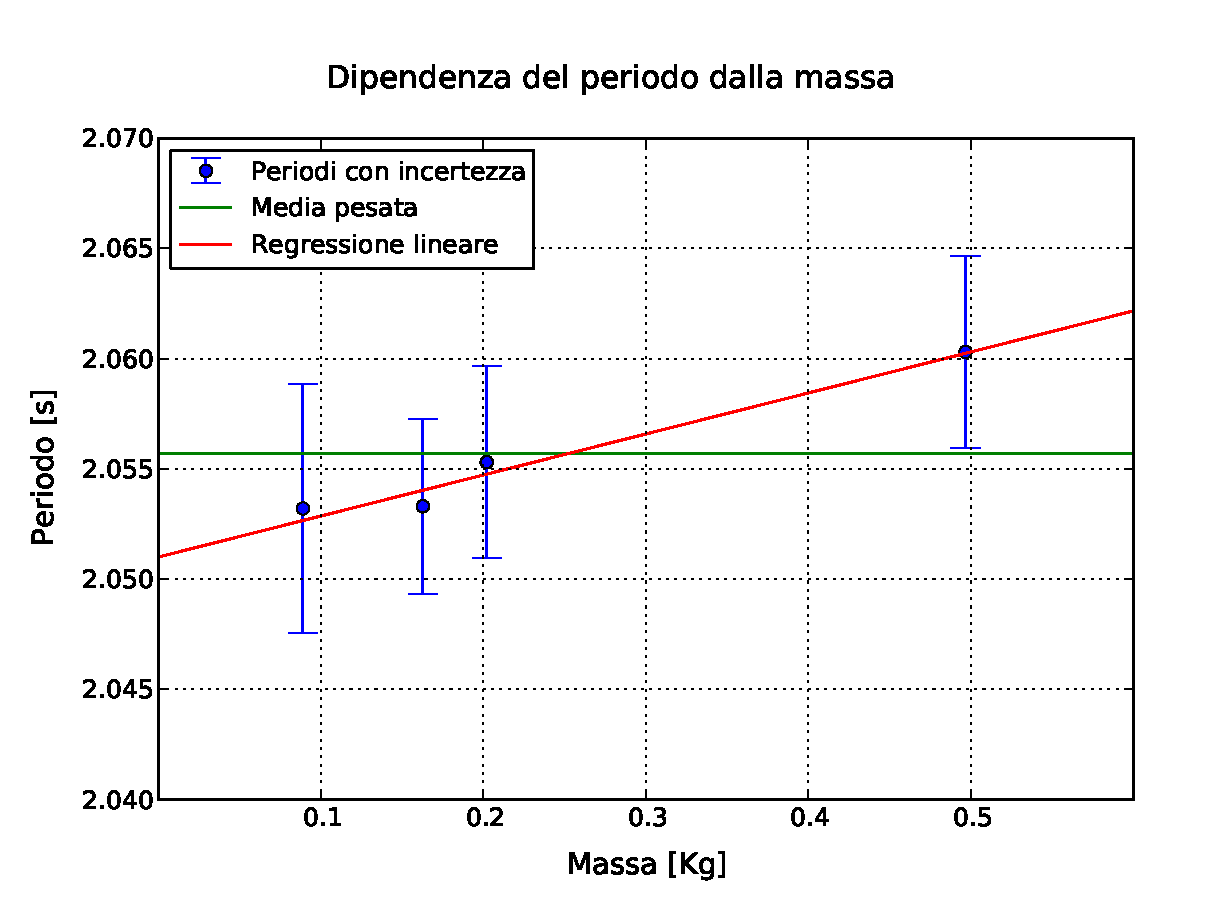
\includegraphics[width=110mm]{immagini/masse.pdf}
    \caption{Il seguente grafico rappresenta sull'asse delle ordinate le medie dei periodi relativi ad ogni
        singola massa, mentre sull'asse delle ascisse sono riportate le masse utilizzate. L'incertezza sul periodo
        è differente da misura a misure, mentre quella reativa alla massa è uguale per tutte, ed in particolare è
        l'incertezza tipo. La retta orizzontale verde rappresenta il valore (costante) della media pesata delle medie
        dei periodi ($\mathcal{T}$), mentre in rosso è rappresentata la retta derivante dalla regressione lineare,
        ovvero la funzione $\mathcal{T} = A + B\,m$.}
    \label{fig: periodo vs masse}
\end{SCfigure}

Finora abbiamo assunta veritiera l'ipotesi che il periodo di oscillazione del pendolo non dipende linearmente dalla massa applicata. Ciononostante ora vogliamo controllare se effettivamente sia così e quindi abbiamo deciso di fare una regressione lineare sulla funzine $f$ in modo da dare una stima ai parametri A e B e verificare che A risulti compatibile con il periodo del pendolo $\mathcal{T}$ trovato grazie alla media pesata e che il valore di B sia compatibie con lo 0 teorico.\\

Procediamo operativamente in questo modo per eseguire la regressione lieare:

\begin{itemize}
	\item{Grazie al grafico sopra riportato (Figura \ref{fig: periodo vs masse}) diamo una stima preliminare dei due parametri A e B: al parametro A è stato associato il valore del periodo $\mathcal{T}$ trovato grazie alla media pesata, mentre per avere una stima del parametro B abbiamo deciso di calcolare il coefficiente angolare della retta che intercetta i dati, ovvero:
			\begin{equation*}
				A \,=\, \mathcal{T}; \quad \quad B \,=\, \frac{\mathcal{T}_4 - \mathcal{T}_1}{m_4 - m_1} \,=\, 0.017165
			\end{equation*}
			%
			}
	\item{La funzione da minimizzare che misura la discrepanza è:
			\begin{equation}
                \sum_{i=1}^{N} \frac{(\mathcal{T}_i - A - B m_i)}{(\delta \mathcal{T}_{tot})^2}	
                \label{eq:min_quad}
			\end{equation}
			%
            dove $\delta \mathcal{T}_{tot}$ è l'incertezza totale sulle misure del periodo, ottenuta sommando l'incertezza $\delta \mathcal{T}_i$ e l'errore trasferito dal peso, che risulta essere però trascurabile rispetto all'incertezza sul periodo poichè $\delta \mathcal{T}_i$ risulta essere dell'ordine di grandezza di $10^{-3}$ mentre l'incertezza trasferita dalla massa è dell'ordine di $10^{-6}$, e quindi quest'ultima risulta essere trascurabile rispetto all'incertezza sul periodo;}
	\item{Quindi per quanto studiato in classe abbiamo che:

			\begin{equation*}
				A \,=\, \frac{(\sum_i w_i m_i^2)(\sum_i w_i \mathcal{T}_i) - (\sum_i w_i m_i)(\sum_i w_i m_i \mathcal{T}_i)}{\Delta} \,=\, 2.0510 \,\, s
			\end{equation*}
			%
			\begin{equation*}
				B \,=\, \frac{(\sum_i w_i)(\sum_i w_i m_i \mathcal{T}_i) - (\sum_i w_i \mathcal{T}_i)(\sum_i w_i m_i)}{\Delta} \,=\, 0.01862
			\end{equation*}
			%
			dove:
			\begin{equation*}
				\Delta \,=\, (\sum_i w_i)(\sum_i w_i m_i^2) - (\sum_i w_i m_i)^2 \,\,\,\,\,\,\, e \,\,\,\,\,\,\,
				w_i \,=\, \frac{1}{(\delta \mathcal{T}_i)^2}
			\end{equation*}}
	\item{Di conseguenza abbiamo che le incertezze relative su A e B sono:

			\begin{equation*}
				(\delta A)^2 \,=\, \frac{\sum_i w_i m_i^2}{\Delta}  \,\,\,\,\, e \,\,\,\,\,
				(\delta B)^2 \,=\, \frac{\sum_i w_i}{\Delta} 
			\end{equation*}}
	\end{itemize} 
	Quindi possiamo riassumere i risultati di questa procedura in questo modo:

	\begin{equation*}
		A \,\pm\, \delta A \,=\, (2.051 \,\, \pm \,\, 0.004) \,\,s \,\,\,\,\, e \,\,\,\,\,
		B \,\pm\, \delta B \,=\, (0.018602 \,\, \pm \,\, 0.014691) \,\,
	\end{equation*}
	WARNING! servono davvero così tante cifre significative su B??? i don't think so... do ya?

	%
Quindi non ci rimane altro che verificare se i due parametri così trovati risultano compatibili con quelli ipotizzati, ovvero A deve risultare compatibile con il periodo medio del pendolo calcolato grazie alla media pesata, mentre B deve risultare compatibile con lo 0 teorico. Pertanto posto a priori un fattore di copertura pari a tre ($k = 3$):

\begin{itemize}
	\item{calcoliamo la discrepanza $R$ tra $\mathcal{T}$ ed A, ottenendo:
			\begin{equation*}
				R \,=\, \mathcal{T} - A \,=\, 0.005 \,s
			\end{equation*}
			%
			}
	\item{verificiamo ora se $R \leq k\,\sigma[R]$, dove:
			\begin{equation*}
				\sigma[R] \,=\, \sqrt{(\delta \mathcal{T})^2 + (\delta A)} \,=\, 0.004  \, s \bigotimes
			\end{equation*}
			%
			pertanto otteniamo che:
			\begin{equation*}
				R \leq k\,\sigma[R] \quad \text{in quanto} \quad 0.005 \, s \leq 0.013 \, s \bigotimes
			\end{equation*}
WARNING! qualcosa non quadra nelle moltiplicazioni, sono giuste?			
			
			%
			e quindi $\mathcal{T}$ risulta compatibile con A}
	\item{troviamo ora la discrepanza $R$ tra $B$ ed il valore teorico 0, ottenendo:
			\begin{equation*}
				R \,=\, B - 0 \,=\, 0.0186
			\end{equation*}
			%
			}
	\item{controlliamo ora se $R \leq k\,\sigma[R]$, dove:
			\begin{equation*}
				\sigma[R] \,=\, \sqrt{(\delta A)^2} \,=\, 0.0147	
			\end{equation*}
			%
			pertanto otteniamo che:
			\begin{equation*}
				R \leq k\,\sigma[R] \quad \text{in quanto} \quad 0.0186 \leq 0.0441
			\end{equation*}
			%
			e quindi $B$ risulta compatibile con lo 0 teorico}			
\end{itemize}
Quindi grazie a questa breve analisi abbiamo trovato che le ipotesi fatte inizialmente risultano essere corrette in quanto abbiamo verificato che il periodo del pendolo non dipende dalla massa applicata, restringendoci a considerare il nostro modello a quello di pendolo semplice e considerando le masse puntiformi.

%A =  2.0510
%B =  0.018602
%sigma_A =  0.0042932
%sigma_B =  0.014691
%chi2_fit =  0.057346
